\chapter{基本的网络命令}
\label{chap:basicNetworkCommands}
\begin{flushleft}
\rule[0mm]{\textwidth}{.1pt}
\end{flushleft}

一个网络是由多台连在一起的计算机构成的。网络可以简单到家里或办公室中相
连的几台计算机,也可以复杂到一个大学的网络或是整个因特网。当我们的计算
机是网络的一部分时,我们就可以访问那些系统,要么是直接访问,要么可以通
过邮件或网页进行访问。

我们可以使用的网络工具有很多,有一些是方便用来诊断网络是否有问题的工具,
另一些(如邮件阅读器或网页浏览器)则是用来完成一些工作或是与他人保持联
系的。

\section{ping}
\label{chap:basicNetworkCommands:ping}

\texttt{ping}(8)的作用是将ICMP的\texttt{ECHO\_REQUEST}报文发送给指定的
主机。如果主机响应了,那么我们就可以收到ICMP的回答报文。听起来很诡异是
吧。好吧,我们可以``ping''一个特定的IP地址来看那个IP地址的主机是不是活
动的。如果没有响应,我们就知道出了点什么毛病。下面是两个Linux用户的对
话。

\begin{quote}
  \texttt{用户A:}Loki又访问不了了。\\
  \texttt{用户B:}你确定?\\
  \texttt{用户A:}对啊,我``ping''了它好久了,都没反应。\\
\end{quote}

像这些例子数不胜数,因此,\texttt{ping}命令在日常生活中是个极为有用的
命令。它为我们提供了快速检查一台机器是否开启并连接到网络上的方法。基本
语法如下:
\begin{Verbatim}[frame=single, commandchars=\\\{\}]
\% \textbf{ping www.slackware.com}
\end{Verbatim}

当然,它还能指定其它的一些选项,照例看它的manm手册吧。

\section{traceroute}
\label{chap:basicNetworkCommands:traceroute}
Slackware的\texttt{traceroute}(8)命令是一个极为有用的网络诊断工具。
\texttt{traceroute}命令会显示一个数据包传送到目的地的过程中经过的所有
主机。例如,你可以使用下面命令查看你的主机距离Slackware官网的``跳数'':
\begin{Verbatim}[frame=single, commandchars=\\\{\}]
\% \textbf{traceroute www.slackware.com}
\end{Verbatim}

这个命令会显示途中的所有主机以及各主机的响应时间。以下是一个输出样例:
\begin{Verbatim}[frame=single, commandchars=\\\{\}]
\% \textbf{traceroute www.slackware.com}
traceroute to www.slackware.com (204.216.27.13), 30 hops max, 40 byte packets
1 zuul.tdn (192.168.1.1) 0.409 ms 1.032 ms 0.303 ms
2 207.171.227.254 (207.171.227.254) 18.218 ms 32.873 ms 32.433 ms
3 border-sf-2-0-4.sirius.com (205.134.230.254) 15.662 ms 15.731 ms 16.142 ms
4 pb-nap.crl.net (198.32.128.20) 20.741 ms 23.672 ms 21.378 ms
5 E0-CRL-SFO-03-E0X0.US.CRL.NET (165.113.55.3) 22.293 ms 21.532 ms 21.29 ms
6 T1-CDROM-00-EX.US.CRL.NET (165.113.118.2) 24.544 ms 42.955 ms 58.443 ms
7 www.slackware.com (204.216.27.13) 38.115 ms 53.033 ms 48.328 ms
\end{Verbatim}

\texttt{traceroute}与\texttt{ping}类似,都是使用ICMP包。同样,其它的参
数请自行查阅man手册。

\section{DNS工具}
\label{chap:basicNetworkCommands:dnsTools}
域名服务(全称为Domain Name Service,简写为DNS)是一个将地址转换协议,
将无意义的域名如``www.slackware.com''转换到有意义的IP地址,如
``64.57.102.34''。计算机并不能将包路由到``www.slackware.com'',但可以
将包路由到该域名对应的IP地址。因此DNS让我们能更好地记住一台计算机。如
果没有DNS,我们只能在脑子里记住一堆IP地址,包括哪个IP对应哪台机器,并
且要假定机器的IP地址是固定的。显然用名字来表示计算机会比用IP地址表示来
得好一些。那我们如何将名字映射为IP地址呢?

\subsection{host}
\label{chap:basicNetworkCommands:dnsTools:host}
\texttt{host}(1)命令就是做这个工作的。\texttt{host}可以将一个域名解析
为IP地址,除此之外它没什么其它功能,但使用起来的确很方便。
\begin{Verbatim}[frame=single, commandchars=\\\{\}]
\% \textbf{host www.slackware.com}
www.slackware.com is an alias for slackware.com.
slackware.com has address 64.57.102.34
\end{Verbatim}

但如果我们知道了一个IP地址,想知道它对应的域名又应该怎么办呢?

\subsection{nslookup}
\label{chap:basicNetworkCommands:dnsTools:nslookup}
\texttt{nslookup}是一个历经岁月,屹立不倒的工具。但现在已经不建议使用
\texttt{nslookup}了,未来的版本中可能会移除这个工具。
\footnote{slackbook 2.0说nslookup连man手册都没有,笔者在Slackware
  13.37中依然可以使用\texttt{man nslookup}(1)查看它的man手册。}
\begin{Verbatim}[frame=single, commandchars=\\\{\}]
\% \textbf{nslookup 64.57.102.34}
Note: nslookup is deprecated and may be removed from future releases.
Consider using the ‘dig’ or ‘host’ programs instead. Run nslookup with
the ‘-sil[ent]’ option to prevent this message from appearing.
Server:       192.168.1.254
Address:      192.168.1.254#53
Non-authoritative answer:
www.slackware.com        canonical name = slackware.com.
Name:    slackware.com
Address: 64.57.102.34
\end{Verbatim}

\subsection{dig}
\label{chap:basicNetworkCommands:dnsTools:dig}
栅栏里最凶猛的恶狗,域名信息获取器\footnote{The meanest dog in the
  pund, the domain information groper.},简称\texttt{dig}(1),是一个挖
掘DNS信息的工具。\texttt{dig}几乎可以获取DNS服务器的任何信息,包括:反
向查询、A、CNAME、MX、SP及TXT记录。\texttt{dig}的选项很多,如果你不熟
悉的话,我们强烈建议你查看它的man手册。
\begin{Verbatim}[frame=single, commandchars=\\\{\}]
\% \textbf{dig @192.168.1.254 www.slackware.com mx}
; <<>> DiG 9.2.2 <<>> @192.168.1.254 www.slackware.com mx
;; global options: printcmd
;; Got answer:
;; ->>HEADER<<- opcode: QUERY, status: NOERROR, id: 26362
;; flags: qr rd ra; QUERY: 1, ANSWER: 2, AUTHORITY: 2, ADDITIONAL: 2

;; QUESTION SECTION:
;www.slackware.com.      IN MX

;; ANSWER SECTION:
www.slackware.com. 76634 IN CNAME slackware.com.
slackware.com. 86400     IN MX 1 mail.slackware.com.

;; AUTHORITY SECTION:
slackware.com. 86400     IN NS ns1.cwo.com.
slackware.com. 86400     IN NS ns2.cwo.com.

;; ADDITIONAL SECTION:
ns1.cwo.com. 163033      IN A 64.57.100.2
ns2.cwo.com. 163033      IN A 64.57.100.3
;;
;;
;;
;;
Query time: 149 msec
SERVER: 192.168.1.254#53(192.168.1.254)
WHEN: Sat Nov 6 16:59:31 2004
MSG SIZE rcvd: 159
\end{Verbatim}

这个例子应该就能让你对\texttt{dig}的工作原理有一个认识。
``@192.168.1.254''的作用是指定使用的DNS服务器。``www.slackware.com''是
我们要查找的域名,``MX''是查找的类型。上述信息告诉我们发送给
``www.slackware.com''的邮件会被送到``mail.slackware.com''来进行投递。

\subsection{finger}
\label{chap:basicNetworkCommands:dnsTools:finger}
\texttt{finger}(1)的作用是获取一个特定用户的信息。给定一个用户名或
email地址,finger会尝试连接必要的服务器,并获取对应的用户名、办公室位
置、电话号码及其它的信息。下面是一个例子:
\begin{Verbatim}[frame=single, commandchars=\\\{\}]
\% \textbf{finger johnc@idsoftware.com}
\end{Verbatim}

\texttt{finger}会返回用户名、邮件状态、电话号码及我们称为``点计划文件
(文件名以点号开头,内容为用户的计划)''和``点项目文件''。当然,
\texttt{finger}服务器不同,返回的信息也不同。默认情况下,Slackware中包
含的\texttt{finger}服务器会返回如下信息:
\begin{itemize}
\item 用户名
\item 用户房间号
\item 家中电话
\item 工作电话
\item 登陆状态
\item Email状态
\item 用户主目录下的\path{.plan}文件
\item 用户主目录下的\path{.project}文件
\end{itemize}
前面四项可以用\texttt{chfn}命令设置。这些信息存储在\path{/etc/passwd}
文件。而修改\path{.plan}及\path{.project}文件的话则只要用文本编辑器进
行编辑即可。

许多用户使用\texttt{finger}来从远端机器上快速查看自己是否有新邮件。或
者,你也可以查看一个用户的计划或现在的项目。

和其它命令一样,\texttt{finger}也有一定的选项,请查看它的man手册。


\section{telnet}
\label{chap:basicNetworkCommands:telnet}
有些人曾声称\texttt{telnet}(1)是它在计算机上见过的最酷的东西。是否能远
程登陆一个机器并有上面做事是区分Unix及类Unix系统与其它操作系统的一个重
要因素。

\texttt{telnet}使我们能远程登陆到一台计算机,就像直接坐在它面前。一旦
我们的用户名和密码都通过检查,我们就能得到一个shell提示符。之后,我们
就能像在其它文本终端中使用一样来操作它。写邮件、阅读新闻组、移动文件等
等。如果我们在X下工作,并用\texttt{telnet}连接到其它机器上,我们可以在
远程机上运行X程序,并在本地显示结果。

用下面的命令来登陆远程服务器:
\begin{Verbatim}[frame=single, commandchars=\\\{\}]
\% \textbf{telnet <hostname>}
\end{Verbatim}
如果该主机响应了,那么我们就能得到一个登陆提示符。输入用户名和密码就OK
了。之后我们就可以在shell环境中为所欲为了。要结束telnet会话,用
\texttt{exit}命令或是\texttt{logout}命令。
\begin{quote}
  \textbf{注意:}\texttt{telnet}并不对传输的信息进行加密。所有传输的内
  容都是纯文本的,连密码也是如此。所以我们并不建议在因特网上使用
  \texttt{telnet},而使用\texttt{Secure Shell}(也称为\texttt{ssh})。
  它对所有信息进行加密并且是免费的。
\end{quote}

\subsection{telnet的其它用法}
\label{chap:basicNetworkCommands:telnet:otherUse}
尽管我们刚刚才说服你不要再用telnet协议来远程登陆,我们还有要介绍
\texttt{telnet}的一些其它用法。

首先,我们可以使用\texttt{telnet}命令从某个特定的端口连接到一个主机上。
\begin{Verbatim}[frame=single, commandchars=\\\{\}]
\% \textbf{telnet <hostname> [port]}
\end{Verbatim}

这在一些情况下是十分方便的,如我们立即需要一个特定的服务,或我们想完全
控制我们使用的命令,或都在我们想观察它的底层运行过程的情况下。我们可以
通过这个方法来交互地对SMTP服务器、POP3服务器或HTTP服务器进行测试或使用。
\begin{Verbatim}[frame=single, commandchars=\\\{\}]
\% \textbf{telnet store.slackware.com 80}
Trying 69.50.233.153...
Connected to store.slackware.com.
Escape character is ’^]’.
HEAD / HTTP/1.0

HTTP/1.1 200 OK
Date: Mon, 25 Apr 2005 20:47:01 GMT
Server: Apache/1.3.33 (Unix) mod_ssl/2.8.22 OpenSSL/0.9.7d
Last-Modified: Fri, 18 Apr 2003 10:58:54 GMT
ETag: "193424-c0-3e9fda6e"
Accept-Ranges: bytes
Content-Length: 192
Connection: close
Content-Type: text/html
Connection closed by foreign host.
\%
\end{Verbatim}

我们也可以对其它的纯文本协议使用这个方法,只要知道它的端口号是多少,及
相应是命令是什么。

\section{The Secure shell}
\label{chap:basicNetworkCommands:ssh}
今天,secure shell获得了当然所有\texttt{telnet}得到过的宠幸。
\texttt{ssh}(1)为我们提供了一种远程登陆的方法,曾经的远在天涯,如今近
在咫尺。然而,\texttt{ssh}对两台机器间传递的所有的数据都进行了加密,那
么,即使第三方拦截了通信,它们也不能获取什么有用的信息。一个典型的ssh
连接如下所示:
\begin{Verbatim}[frame=single, commandchars=\\\{\}]
\% \textbf{ssh carrier.lizella.net -l alan}
The authenticity of host ’carrier.lizella.net (192.168.1.253)’ can’t be
established.
RSA key fingerprint is 0b:e2:5d:43:4c:39:4f:8c:b9:85:db:b2:fa:25:e9:9d.
Are you sure you want to continue connecting (yes/no)? yes
Warning: Permanently added ’carrier.lizella.net’ (RSA) to the list of
known hosts.
Password: \textbf{password}
Last login: Sat Nov 6 16:32:19 2004 from 192.168.1.102
Linux 2.4.26-smp.
alan@carrier:~\$ \textbf{ls -l MANIFEST}
-rw-r--r-- 1 alan users 23545276 2004-10-28 20:04 MANIFEST
alan@carrier:~\$ \textbf{exit}
logout
Connection to carrier.lizella.net closed.
\end{Verbatim}
正如我们看到的,我们用ssh连接到\path{carrier.lizella.net},并检查
\texttt{MANIFEST}文件的权限。

\section{email}
\label{chap:basicNetworkCommands:email}
发送电子邮件是上网后能做的许多有趣的事之一。1998年,有报道说人们发送的
电子邮件比传统的邮件要更多。现在当然更是如此,可见它是很常见并很有用的。

Slackware下,我们提供了一个标准的邮件服务器及好几个邮件客户端。我们这
里讨论的所有客户端都是基于文本的。有许多Windows用户反对基本文本的客户
端,但你会发现基本文本的客户端很方便,尤其是远程查看邮件的时候。不过不
要害怕,Slackware同时提供了一些图形界面的电子邮件客户端如Thunderbird及
KDE的Kmail等。如果你想使用它们的话,请查看帮助菜单。当然,现在许多电子
邮件提供商提供了相应的网页接口可供使用。


\subsection{pine}
\label{chap:basicNetworkCommands:email:pine}
\texttt{pine}与\texttt{elm}不同\footnote{pine的意思是松树,elm则为榆树,
  但它们同时又代表两个不同的邮件客户端,也可译为,松是松,榆是榆。}。
或者有类似的说法。\texttt{pine}是现存的最古老的命令行邮件客户端之一,
也是最友好的客户端之一。\texttt{pine}是华盛顿大学创建的,在发布的时候
也附带了它的商标及版权许可,所以不好使用。幸运的是在2005年,华盛顿大学
觉得有必要重新写一款没有商标,许可更开放的pine,于是\texttt{alpine}(1)
就诞生。这也是在Slackware上使用的pine。要使用它,只要在命令行中输入
pine即可。它的使用很简单,主要是因为它是菜单驱动的,同时在屏幕底端显示
了可以使用的命令。你还是自己看看吧。
\begin{figure}[htpb]
  \centering
  
\begin{Verbatim}[frame=single, commandchars=\\\{\}]
  ALPINE 2.00   MAIN MENU              Folder: INBOX               No
Messages  


          ?     HELP               -  Get help using Alpine           

          C     COMPOSE MESSAGE    -  Compose and send a message      

          I     MESSAGE INDEX      -  View messages in current folder 

          L     FOLDER LIST        -  Select a folder to view         

          A     ADDRESS BOOK       -  Update address book             

          S     SETUP              -  Configure Alpine Options        

          Q     QUIT               -  Leave the Alpine program        


                  Copyright 2006-2008 University of Washington
                    [Folder "INBOX" opened with 0 messages]
? Help                     P PrevCmd                 R RelNotes                 
O OTHER CMDS > [ListFldrs] N NextCmd                 K KBLock    
\end{Verbatim}

  \caption{pine操作界面}
  \label{fig:pine}
\end{figure}

我们可以看到一个命令菜单以及底部的命令键。\texttt{pine}是个很复杂的软
件,这里,我们只讨论简单的功能。

键入\texttt{i}来查看收件箱的内容。我们的信息是按时间、作者及主题列出的。
高亮想查看的信息并按回车即可查看。而按\texttt{r}键则为回复该邮件。写完
一则邮件后可以按\texttt{Ctrl+X}来发送,按\texttt{i}可以回到信息列表。

要想删除一封信息,请按\texttt{d}键。它会删除当前高亮显示的信息。
\texttt{pine}会在我们退出\texttt{pine}时删除邮件。\texttt{pine}可以让
我们将邮件存储在文件夹中,按下\texttt{l}键可以得到一个文件夹列表。在显
示信息时,按下\texttt{s}键能将其存放到其它文件夹中,它会询问你要存放的
文件夹名,之后将信息存放到相应文件夹中。

\texttt{pine}提供了许多许多的功能,要是你想使用它,一定要看一看它的man
手册。它会包含\texttt{pine}的最新信息。

不要觉得\texttt{pine}过时,当前主流的邮件它都支持,包括gmail。

\subsection{elm}
\label{chap:basicNetworkCommands:email:elm}

\texttt{elm}(1)是另一个流行的基于文本的邮件客户端。尽管它并不如
\texttt{pine}友好,但它的绝对存在了更长的时间。

由于Slackbook 3中似乎已经放弃了对它的介绍,这里也只点到为止。

\subsection{mutt}
\label{chap:basicNetworkCommands:email:mutt}
``所有的邮件客户端都是垃圾,mutt只是更不垃圾一点''。\texttt{mutt}最初
的接口是基于\texttt{elm}的,只是加上了其它邮件客户端的一些功能,结果就
是杂交的mutt。
\texttt{mutt}的一些功能包括:
\begin{itemize}
\item 颜色支持
\item 多线程
\item MIME及PGP/MIME支持
\item pop3及imap的支持
\item 支持多种邮箱格式(mbox、MMDF、MH及maildir等)
\item 高度可定制性
\end{itemize}

\texttt{mutt}的友好程度不如\texttt{pine}(毕竟是基于\texttt{elm}的),
但它的功能更强大,我们在mutt的底部找不到命令提示行,mutt已经把每寸土地
都用来处理邮件了。它支持的特性也是很广泛的。我们可以通过
主目录下的\texttt{.muttrc}文件来配置\texttt{mutt}。由于可定制的东西太
多了,人们甚至专门为它建了一个man手册页:\texttt{muttrc}(5)。你可能会
想读一读。
\begin{Verbatim}[frame=single, commandchars=\\\{\}]
3172 N   Jan 17 Thomas Morper   (2.8K)     │ └─>Re: [Slackbuilds-users] Exim Sbo
3173 N   Jan 17 TuxaneMedia     (2.5K)     └─>Re: [Slackbuilds-users] Exim Sbo
3174 N   Jan 06 Uli Sch?fer     (4.6K) [Slackbuilds-users] mrtg-2.15.2 breaks wi
3175 N   Jan 06 Willy Sudiarto  (4.0K) └─>
3176 N   Jan 06 Audrius Ka??uka (3.9K)   └─>
3177 N   Jan 06 Niels Horn      (4.4K)     └─>
3178 N * Jan 09 King Beowulf    (6.5K) [Slackbuilds-users]  libreoffice (3.3.0rc
3179 N * Jan 09 Niels Horn      (4.8K) └─>Re: [Slackbuilds-users] libreoffice (3
3180   * Jan 09 Niels Horn      (  73)   └─>                                    
3181 N * Jan 09 King Beowulf    (5.9K)     └─>
3182 N   Jan 10 Robby Workman   (7.8K) [Slackbuilds-users] Updates - 20110110
3183 N   Jan 10 B Watson        (3.6K) [Slackbuilds-users] Fwd: nted slackbuild
3184 N   Jan 11 SlackBuilds@cat (2.5K) [Slackbuilds-users] /usr/share/ package s
3185 N   Jan 11 Robby Workman   (3.4K) └─>
3186 N   Jan 12 SlackBuilds@cat (3.4K)   └─>
3187 N   Jan 11 Robby Workman   (4.5K)     └─>
3188 N   Jan 12 Robby Workman   (2.3K) [Slackbuilds-users] Unavailability of mai
3189 N   Jan 13 Mr. B-o-B       (3.7K) └─>
3190 N   Jan 13 Josiah Boothby  (3.2K) [Slackbuilds-users] Ted's Word Processor
3191 N   Jan 14 Adam Swift      (7.4K) [Slackbuilds-users] Web submission failur
3192 N   Jan 14 Rob McGee       (3.5K) └─>
\end{Verbatim}

\subsection{nail}
\label{chap:basicNetworkCommands:email:nail}
有些人连菜单驱动的软件都不想用,就只想用命令行。\texttt{nail}就是一个
命令行驱动的邮件客户端,它很原始,也几乎没有提供什么用户接口。然而,如
果你想快速地写些邮件、用脚本编写一个邮件群发器或是测试MTA的安装或一些
其它类似的工作,那么mailx还是很方便的。注意Slackware为\texttt{nail}创
建了一些符号链接:\path{/usr/bin/mail}及\path{/usr/bin/mailx}。这些命
令执行的都是同一个软件。事实上,一般我们看到的\texttt{nail}都以
\texttt{mail}称呼。

基本的命令如下:
\begin{Verbatim}[frame=single, commandchars=\\\{\}]
\% \textbf{mailx <subject> <to-addr>}
\end{Verbatim}

\texttt{mailx}会从标准输入中读取邮件的正文。所以我们可以用\texttt{cat}
将一个文件写入\texttt{mailx}并发送,或者可以自己写,写完后按
\texttt{Ctrl+D}结束。

下面是个将某个源代码文件通过邮件发送给另一个人:
\begin{Verbatim}[frame=single, commandchars=\\\{\}]
\% \textbf{cat randomfunc.c | mail -s ``Here's that function'' asdf@example.net}
\end{Verbatim}

还想了解更多的话,请参阅man手册。

\section{浏览器}
\label{chap:basicNetworkCommands:browsers}
多数人一听到因特网,立马想到的就是``上网''。或者说是使用网页浏览器浏览
网页。对于一般用户,这或许是因特网最大的功能。

Slacwkare在``XAP''系列中提供了一些流行的图形网页浏览器,而在``N''系统
中包含了一些字符模式下的浏览器。我们会对其中的一些作简要的介绍。

\subsection{lynx}
\label{chap:basicNetworkCommands:browsers:lynx}
要说Slackware中包含的最古老的基于文本终端的浏览器,那么绝对是
\texttt{lynx}(1)。对于查看一些有限的网页信息而言,lynx是十分合适的。但
lynx并不支持网页框架、javascript或图片,它只是一个基于文本的浏览器。它
主要通过键盘进行导航,当然也可以使用鼠标。由于它不支持很多现今的网页特
性,因此lynx是我们可以用于收集信息的速度最快的浏览器。例如,为lynx传递
[-dump]参数会直接将格式化好的网页直接传递给终端,之后就可以通过管道传
递给其它程序。

在提示符下输入\texttt{lynx}即可启动\texttt{lynx}:
\begin{Verbatim}[frame=single, commandchars=\\\{\}]
\% \textbf{lynx}
\end{Verbatim}
例如,想访问google.com,可以为\texttt{lynx}指定参数:
\begin{Verbatim}[frame=single, commandchars=\\\{\}]
\% \textbf{lynx www.google.com}
\end{Verbatim}

\begin{figure}[htpb]
  \centering
  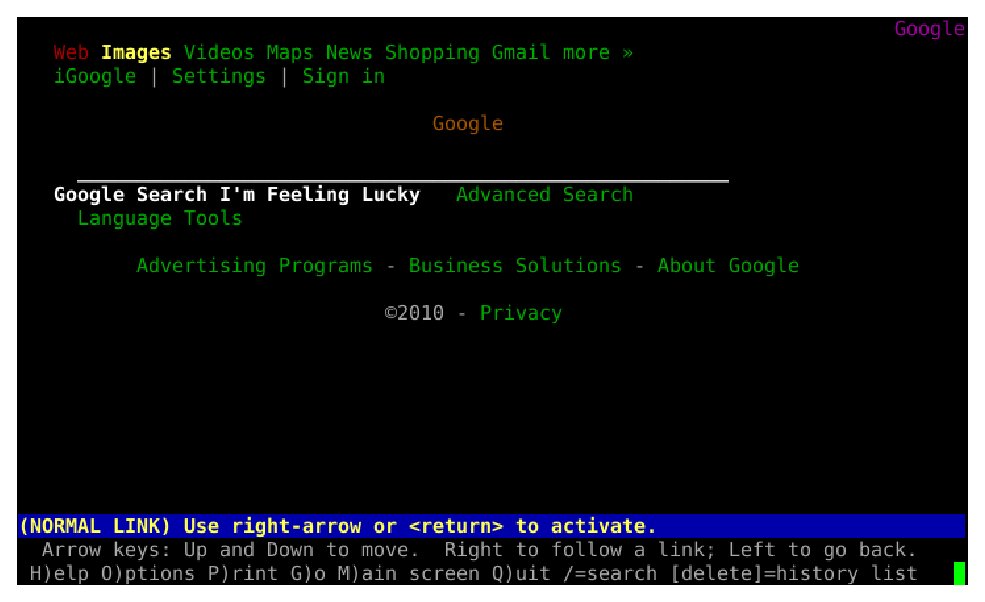
\includegraphics[width=0.85\textwidth]{images/basic-network-commands/lynx.eps}
  \caption{lynx}
  \label{fig:lynx}
\end{figure}
\texttt{lynx}在屏幕下方会给出可以使用的键盘快捷键。上下方向键用于在文
档中移动,回车则会跳转到当前高亮的链接,左方向键则用于回到上一页。而
\texttt{d}键则会下载当前选中的文件。\texttt{g}键会给出提示信息,输入网
址后则跳到输入的网址。

其它的命令要么可以查看man手册,要么可以在\texttt{lynx}中按\texttt{h}键
查看。

\subsection{links}
\label{chap:basicNetworkCommands:browsers:links}
我们还可以选择使用\texttt{links}(1),它是一个基于终端的网页浏览器,支
持网页框架,生成也比lynx要快一些。和在它之前的一些浏览器一样,
\texttt{links}也是使用方向键导航的,当然,同样支持鼠标。与
\texttt{lynx}不同的是,\texttt{links}还包含了一个方便的菜单(只要用鼠
标在屏幕顶端点击即可。),显示也要好一些。
\begin{figure}[htpb]
  \centering
  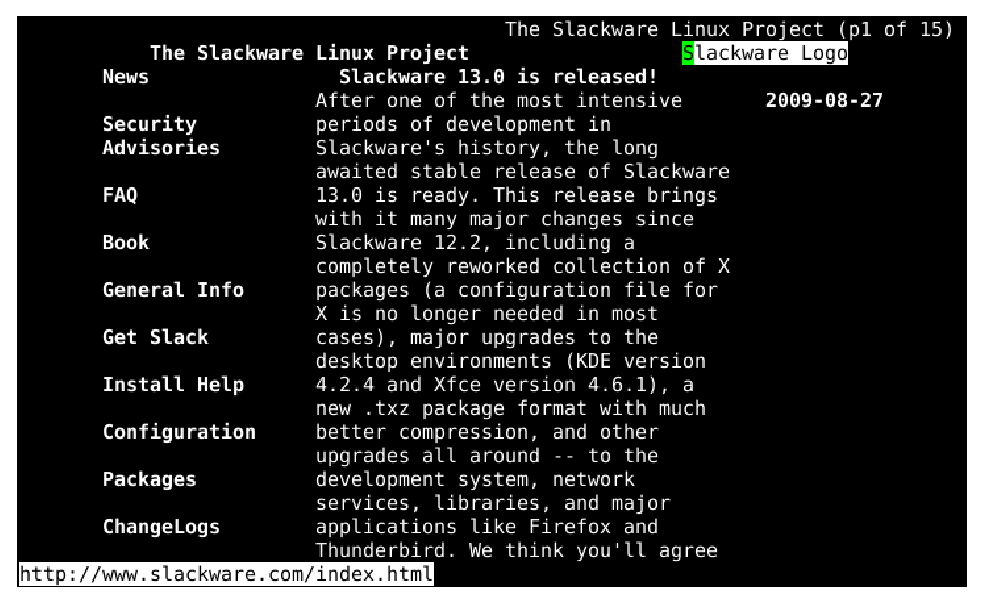
\includegraphics[width=0.85\textwidth]{images/basic-network-commands/links.eps}
  \caption{links}
  \label{fig:links}
\end{figure}

\subsection{wget}
\label{chap:basicNetworkCommands:browsers:wget}
与我们前面介绍的浏览器不同,\texttt{wget}(1)是非交互式的。
其它的浏览器是显示HTTP的内容,而\texttt{wget}则是下载这些内容。这是一
种不在浏览器中``浏览''网页的方法。与其它浏览器的dump模式不同,
\texttt{wget}不对下载的内容进行格式修改。它只是原封不动地从网页服务器
上复制所有的标签及二进制文件。它还支持递归选项,可以用来在本地对网上的
某些内容做镜像。\texttt{wget}不仅仅对HTTP内容有效,它还支持FTP及其它的
协议。
\begin{Verbatim}[frame=single, commandchars=\\\{\}]
darkstar:~# \textbf{wget \textbackslash{}}
\textbf{ftp://ftp.osuosl.org/pub/slackware/slackware-current/ChangeLog.txt}
--2010-05-01 13:51:19--
ftp://ftp.osuosl.org/pub/slackware/slackware-current/ChangeLog.txt
           => `ChangeLog.txt'
Resolving ftp.osuosl.org... 64.50.236.52
Connecting to ftp.osuosl.org|64.50.236.52|:21... connected.
Logging in as anonymous ... Logged in!
==> SYST ... done.    ==> PWD ... done.
==> TYPE I ... done.  ==> CWD /pub/slackware/slackware-current ...  done.
==> SIZE ChangeLog.txt ... 75306
==> PASV ... done.    ==> RETR ChangeLog.txt ... done.
Length: 75306 (74K)

100\%[======================================>] 75,306       110K/s   in 0.7s    

2010-05-01 13:51:22 (110 KB/s) - `ChangeLog.txt' saved [75306]
\end{Verbatim}

\texttt{wget}有许多选项,这使得它在应用于网站的脚本中十分方便(镜像网
络或其它工作)。最好还是查看它的man手册以了解它的用法。

\section{FTP客户端}
\label{chap:basicNetworkCommands:ftp}
FTP全称为File Transfer Protocol,译为文件传输协议。它使我们能在两台机
器间发送接收文件。FTP协议包括FTP服务器和FTP客户端。本节只讨论客户端。

简单的说,客户端就是我们自己,服务器就是响应我们请求的远程机器。我们会
从服务器上下载文件或上传文件到服务器上,而客户端并不支持其它客户端的
FTP连接,它只能用来连接到其它服务器。

\subsection{ftp}
\label{chap:basicNetworkCommands:ftp:ftp}
连接到FTP服务器的最方便的方法是执行\texttt{ftp}(1)命令,并指定要连接的
主机名:
\begin{Verbatim}[frame=single, commandchars=\\\{\}]
\% \textbf{ftp <hostname> [port]}
\end{Verbatim}

如果该主机上运行着一个FTP服务器,那么它会询问用户名及密码。我们可以以
自己的用户名登陆,或者使用``anonymous''用户名,匿名登陆对于存放软件归
档的一些服务器十分流行。例如,我们想通过FTP获得Slackware,那么就可以使
用匿名FTP。

一旦登陆了,我们就会看到\texttt{ftp>}提示符。FTP有自己的命令,但和标准
的命令类似,下面列出了一些基本的命令及作用:
\begin{table}[htpb]
  \centering
  \begin{tabular}{l|l}
    \hline \hline
    命令 & 作用 \\ \hline
    \texttt{ls} & 列出文件 \\
    \texttt{cd <dirname>} & 改变当前工作目录 \\
    \texttt{bin} & 设置为二进制传输模式 \\
    \texttt{ascii} & 设置为ASCII传输模式 \\
    \texttt{get <filename>} & 下载文件 \\
    \texttt{put <filename>} & 上传文件 \\
    \texttt{hash} & 开关hash标记 \\
    \texttt{tick} & 开关字节计数器 \\
    \texttt{prom} & 为下载开启交互模式 \\
    \texttt{mget <mask>} & 下载一个文件或一组文件,可以使用通配符 \\
    \texttt{mput <mask>} & 上传一个文件或一组文件,可以使用通配符 \\
    \texttt{quit} & 退出FTP服务器 \\
    \hline \hline
  \end{tabular}
  \caption{ftp命令}
  \label{tab:ftp-commands}
\end{table}

我们还可以使用下面这些命令:\texttt{chmod}、\texttt{delete}、
\texttt{rename}、\texttt{rmdir}等。这些命令可以看名知意,不多解释。想
查看ftp支持的所有命令,可以在\texttt{ftp>}提示符下输入\texttt{help}或
\texttt{?}。

FTP是一个相对简单的程序,但缺少了现在我们日常生活中使用的一些用户接口,
ftp(1)的man手册中对其中的一些命令行参数进行了讲解。
\begin{figure}[htpb]
  \centering
  
\begin{Verbatim}[frame=single, commandchars=\\\{\}]
ftp> \textbf{ls *.TXT}
200 PORT command successful.
150 Opening ASCII mode data connection for /bin/ls.
-rw-r--r-- 1 root 100 18606 Apr 6 2002 BOOTING.TXT
-rw-r--r-- 1 root 100 10518 Jun 13 2002 COPYRIGHT.TXT
-rw-r--r-- 1 root 100 602 Apr 6 2002 CRYPTO_NOTICE.TXT
-rw-r--r-- 1 root 100 32431 Sep 29 02:56 FAQ.TXT
-rw-r--r-- 1 root 100 499784 Mar 3 19:29 FILELIST.TXT
-rw-r--r-- 1 root 100 241099 Mar 3 19:12 PACKAGES.TXT
-rw-r--r-- 1 root 100 12339 Jun 19 2002 README81.TXT
-rw-r--r-- 1 root 100 14826 Jun 17 2002 SPEAKUP_DOCS.TXT
-rw-r--r-- 1 root 100 15434 Jun 17 2002 SPEAK_INSTALL.TXT
-rw-r--r-- 1 root 100 2876 Jun 17 2002 UPGRADE.TXT
226 Transfer complete.
ftp> \textbf{tick}
Tick counter printing on (10240 bytes/tick increment).
ftp> \textbf{get README81.TXT}
local: README81.TXT remote: README81.TXT
200 PORT command successful.
150 Opening BINARY mode data connection for README81.TXT (12339 bytes).
Bytes transferred: 12339
226 Transfer complete.
12339 bytes received in 0.208 secs (58 Kbytes/sec)
\end{Verbatim}
  \caption{ftp示例}
  \label{tab:ftp-examples}
\end{figure}

\subsection{ncftp}
\label{chap:basicNetworkCommands:ftp:ncftp}
\texttt{ncftp}(1)(发音为``Nik-F-T-P'')是另一个Slackware自带的ftp客户
端。它仍旧是个基于文本的程序,但比\texttt{ftp}多了许多功能,包括:
\begin{itemize}
\item TAB补全
\item 为文件添加书签
\item 支持更多的通配符
\item 保存命令历史
\end{itemize}

默认情况下,\texttt{ncftp}会尝试匿名登陆我们指定的服务器。通过传递
``\texttt{-u}''参数,我们可以强制让\texttt{ncftp}显示一个登陆提示符。
一旦登陆后,我们就可以使用与\texttt{ftp}相同的命令。区别就是它的接口更
为友好,感觉像在用\texttt{bash}一样。
\begin{Verbatim}[frame=single, commandchars=\\\{\}]
ncftp /pub/linux/slackware > \textbf{cd slackware-current/}
Please read the file README81.TXT
  it was last modified on Wed Jun 19 16:24:21 2002 - 258 days ago
CWD command successful.
ncftp ...ware/slackware-current > \textbf{ls}
BOOTING.TXT                FAQ.TXT                       bootdisks/
CHECKSUMS                  FILELIST.TXT                  extra/
CHECKSUMS.asc              GPG-KEY                       isolinux/
CHECKSUMS.md5              PACKAGES.TXT                  kernels/
CHECKSUMS.md5.asc          PRERELEASE\_NOTES              pasture/
COPYING                    README81.TXT                  rootdisks/
COPYRIGHT.TXT              SPEEKUP\_DOCS.TXT              slackware/
CRYPTO\_NOTICE.TXT          SPEEK\_INSTALL.TXT             source/
CURRENT.WARNING            Slackware-HOWTO 
ChangeLog.txt              UPGRADE.TXT
ncftp ...ware/slackware-current > \textbf{get README81.TXT}
README81.TXT:                                          12.29 kB 307.07 kB/s
\end{Verbatim}


\section{与其它用户交谈}
\label{chap:basicNetworkCommands:talk}

\subsection{wall}
\label{chap:basicNetworkCommands:talk:wall}
\texttt{wall}(1)命令是一个向同一系统的其它用户传递信息的快速方法。基本
的语法为:
\begin{Verbatim}[frame=single, commandchars=\\\{\}]
\% \textbf{wall [file]}
\end{Verbatim}

这个命令的结果就是[file]中的内容会显示在所有当前登陆用户的终端屏幕上。
如果不指定一个文件,那么\texttt{wall}会从标准输入中读取信息,我们只要
输入信息即可,按\texttt{Ctrl+d}结束。

\texttt{wall}命令没什么其它功能,它只是用来告诉当前的用户,我们要对系
统做一些重要的维护工作,可能还要重启,所以你们最好先保存一下现在的工作,
然后就登出吧。

\subsection{talk}
\label{chap:basicNetworkCommands:talk:talk}
\texttt{talk}(1)命令能让两个用户交谈。它水平地将屏幕分割成两部分。请求
与另一个用户对话,使用如下命令:
\begin{Verbatim}[frame=single, commandchars=\\\{\}]
\% \textbf{talk <persion> [ttyname]}
\end{Verbatim}

如果我们只指定了用户名,则该对话假设是在本地进行的,所以只查询本地的用
户。如果我们想与某个特定tty上的用户(如果用户从不同的tty登陆)交谈,则
要指定\texttt{ttyname}参数。\texttt{talk}所需要的信息可以通过
\texttt{w}命令得到。

\texttt{talk}也可以访问远程的用户。至于用户名,可以简单地填上一个邮件
地址,\texttt{talk}会尝试联系对应主机上的用户。

\texttt{talk}功能有限。它只支持两个用户并且是半双工的。

\subsection{ytalk}
\label{chap:basicNetworkCommands:talk:ytalk}
\texttt{ytalk}(1)与\texttt{talk}向后兼容。Slackware中两个命令都有。它
们的语法也类似,只有一些微小的区别:
\begin{Verbatim}[frame=single, commandchars=\\\{\}]
\% \textbf{ytalk <username> [#ttyname]}
\end{Verbatim}

用户名及ttyname参数与\texttt{talk}一样,除了要加一个\#号。

\texttt{ytalk}改进的地方有:
\begin{itemize}
\item 它支持两个以上的用户
\item 可以用Esc键唤出菜单来选择一些选项。
\item 在使用talk会话时还能使用shell
\item 还有一些其它的……
\end{itemize}
要使用\texttt{ytalk},必须在\path{/etc/inetd.conf}文件中开启
\texttt{ntalk}端口,否则\texttt{ytalk}无法正常工作。

%TODO: add rsync as in Slackbook 3

%%% Local Variables: 
%%% mode: latex
%%% TeX-master: "../SlackGuide"
%%% End: 
